\chapter{Generación del documento de texto}

\section{Diseño}
El documento de texto debe contener toda la información de la ontología, organizado en secciones, subsecciones y párrafos. Para alcanzar el documento final, se crearon módulos teniendo como referencia las actividades de la generación de lenguaje natural nombradas en la Sección \ref{sec:tareas_gnl}. Los tres módulos principales son \emph{macroplanificación}, \emph{microplanificación} y \emph{realización}. Dentro de cada módulo se desarrollaron submódulos, para resolver cada problema específico. 

Si bien en el capítulo anterior se propuso un flujo lineal de información en el organizador de información, en este capítulo, al desarrollar la macroplanificación, se integraron los módulos del organizador de información con los submódulos de la macroplanificación, generando una interacción cíclica entre los módulos. El motivo de esta integración es evitar la creación de interfaces entre los módulos, y el overhead que estas suponen, ya que la creación del árbol de información y la macroplanificación resultan ser procesos equivalentes, por lo que pueden realizarse al mismo tiempo, evitando recorrer el doble de veces la estructura jerárquica. 

En la figura \ref{fig:modulos_plan_documento} se puede ver la integración de los módulos. Los pasos de la interacción entre los módulos se encuentran enumerados en orden, siendo los pasos 5 y 6 repetibles hasta que no hayan más grupos de entidades (correspondientes a niveles en la jerarquía de la estructura).

\begin{figure}[H]
    \centering
    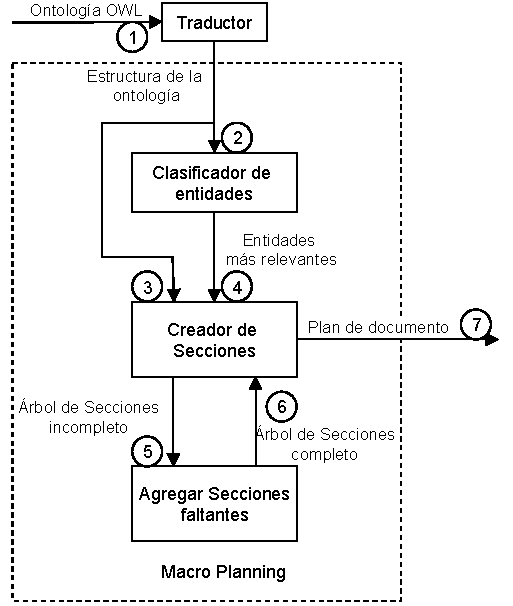
\includegraphics[width=12cm, height=5cm]{img/generacion_documento/modulos_plan_documento.pdf}
    \caption{Integración de módulos para la generación del plan de documento.}
    \label{fig:modulos_plan_documento}
\end{figure}

Cabe aclarar que, si bien la estructuración del documento se determina con base en el árbol de entidades, en el documento final la realización de la estructura (secciones y párrafos) se retrasa hasta tener mayor información acerca de su contenido, es decir, luego de la etapa de microplanificación. Estas tareas se encuentran desarrolladas en los módulos de microplanificación y realización, los cuales se muestran en la figura \ref{fig:modulos_documento_final}.

\begin{figure}[H]
    \centering
    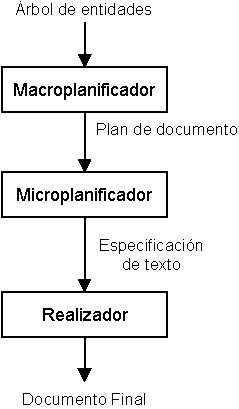
\includegraphics[width=12cm]{img/generacion_documento/modulos_documento_final.pdf}
    \caption{Módulos para la generación del documento final.}
    \label{fig:modulos_documento_final}
\end{figure}

\section{Diseño macro planning}
En esta tarea se planificará la estructura del documento. Como nombramos anteriormente, la organización a priori de la información, realizada en el capítulo anterior, facilita la tarea de macro planificación. Por este motivo, se decidió hacer una arquitectura monolítica entre el organizador de información y el macroplanificador. Sin embargo, para evitar seguir trabajando con árboles de entidades, se construyó un conjunto de componentes para comenzar con el documento de texto. De esta manera, el plan de documento, representado en la figura \ref{fig:modulos_plan_documento} con el número 9, se corresponde a un conjunto de clases que definen una representación interna de un documento de texto. 

Esta representación prepara el terreno para que, luego de la microplanificación, el realizador decida el diseño final del documento.

La creación de la representación interna del documento de texto tiene en cuenta los siguientes criterios:
\begin{itemize}
    \item A cada \emph{OWL:Class} le corresponde una sección.
    \item Cada sección está compuesta de al menos un párrafo y un título.
    \item Cada párrafo trata un único tópico, el cual puede ser una clase o un individuo. También, un párrafo puede o no tener alguna sentencia. Este criterio se debe a que no todas las entidades tienen asociados axiomas que la describan.
    \item Una \emph{owl:ObjectProperty} solo puede ser tópico en una sección cuando agrupa información de la clase correspondiente a esa sección. 
\end{itemize}

\subsection{Diagrama de clases}
En la figura \ref{fig:diagrama_clases_macroplanificador} se muestra el diagrama de clases correspondiente al macroplanificador. El componente principal que integra el macroplanificador con el organizador de información es la clase TextManager. Esta clase se encarga de crear la clase Text, que es la representación interna de un documento de texto. El documento está compuesto por Secciones, Párrafos y Sentencias. Cada Sentencia tiene asociada entidades \emph{OWL} que describen a un único tópico.

\begin{figure}[H]
    \centering
    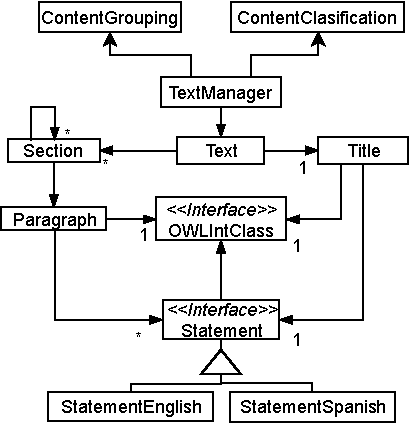
\includegraphics[width=10cm, height=7cm]{img/generacion_documento/diagrama_clases_macroplanificador.pdf}
    \caption{Diagrama de clases del generador del documento de texto.}
    \label{fig:diagrama_clases_macroplanificador}
\end{figure}

\section{Implementación macro panning}

\section{Diseño micro planning}
%El objetivo de esta etapa es organizar el contenido de cada axioma para crear una sentencia gramaticalmente aceptable.
En esta estapa se llevarán a cabo las tareas para describir una entidad en lenguaje natural a partir de los axiomas que la describen en la ontología. Esta descripción en lenguaje natural se alcanza a través de uno o varias oraciones producidas con una estructura que se adapte a la gramática del lenguaje español.

Como existen diversas estructuras sintácticas para expresar un mismo contenido, a modo de simplificación se asoció a cada constructor OWL solo algunas formas de verbalización. Se trató de generar oraciones que sean fieles al significado expresado en los axiomas y de evitar ambigüedades.

Para poder trabajar con patrones de la gramática del lenguaje español, se utilizó un \emph{POS Tagger} para etiquetar las palabras de las definiciones de las clases.

\subsection{Verbalización de la definición de una Clase}
Se decidió definir a cada Clase en lenguaje natural a partir de los axiomas que la describen y agregando además las propiedades en las que participa como dominio.

Esta etapa se divide en tres tareas principales:
\begin{itemize}
    \item Verbalizar los constructores OWL.
    \item Eliminar información redundante entre oraciones a través del proceso de agragación.
    \item Reemplazar con expresiones de referencia a los nombres de las Clases en oraciones consecutivas evitando que se repitan y que genere un texto poco fluido.
\end{itemize}

\subsection{Sintaxis OWL 2}
\label{sec:gen_doc_sintaxis_owl}
Teniendo en cuenta la estructura jerárquica de la sintaxis (a partir de su gramática BNF y de los diagramas de clases de su documentación~\cite{OWL2W3C}), agrupamos en diferentes niveles de abstracción las tres categorías sintácticas: en el nivel inferior se encuentran las Entidades, en el nivel intermedio las Expresiones de Clases, y en el nivel superior los Axiomas. Esta separación en niveles de abstracción será útil para organizar la verbalización. El conjunto de constructores elegido para verbalizar se encuentra en las siguientes listas: en la lista~\ref{list:constructores_axiomas} se agrupan los constructores del nivel de Axiomas, en la lista~\ref{list:constructores_expresiones} los constructores de Expresiones de Clases y en la lista~\ref{list:constructores_entity} los constructores de nivel de Entidades.
\begin{figure}
\begin{multicols}{2}
\captionof{listCap}{Constructores de Entidades}
\label{list:constructores_entity}
    \begin{itemize}
        \item owl:class
        \item owl:objectProperty
        \item owl:dataProperty
        \item owl:individual
        \item[\vspace{\fill}]
    \end{itemize}

\captionof{listCap}{Constructores de Axiomas}
\label{list:constructores_axiomas}
    \begin{itemize}
        \item rdfs:subClassOf
        \item owl:equivalentClass
        \item owl:disjointWith
        \item rdfs:domain
        \item rdfs:range
    \end{itemize}
    \end{multicols}
\end{figure}


\begin{figure}
\captionof{listCap}{Constructores de Expresiones de Clase}
\label{list:constructores_expresiones}
    \begin{itemize}
    \begin{multicols}{2}
        \item owl:intersectionOf
        \item owl:unionOf
        \item owl:complementOf
        \item owl:allValuesFrom
        \item owl:someValuesFrom 
        \item owl:minCardinality
        \item owl:maxCardinality
        \item owl:Cardinality
        \item owl:oneOf
        \item owl:hasValue
        \end{multicols}
    \end{itemize}
\end{figure}

\subsection{Orden de la verbalización}
Ordenaremos la verbalización basados en la separación en niveles de abstracción presente en la Sección~\ref{sec:gen_doc_sintaxis_owl}. 

El enfoque adoptado para crear la sintaxis de las oraciones se basa en un recorrido bottom-up de la jerarquía de un Axioma, construyendo oraciones parciales a partir de los constructores de Expresiones de Clases y de Entidades, hasta alcanzar la raíz de la jerarquía, donde se termina de construir la oración final. 

Con el objetivo de comenzar a formar las oraciones parciales, el primer paso a realizar es verbalizar las Entidades, ya que están directamente relacionadas con las IRIs (o tienen acceso al \emph{label}, en caso de extraer los nombres desde los \emph{labels}).

En la Gramática~\ref{gram:entity} se muestra una porción de la gramática BNF del lenguaje OWL 2 asociada a las entidades.
\begin{GrammarEnv}
%detecta un error de sintaxis pero es mentira.
\begin{grammar}
[(colon){$\rightarrow$}]
[(semicolon)$|$]
[(comma){}]
[(period){\vspace{0.3cm} \\}]
[(quote){\begin{bf}}{\end{bf}}]
[(nonterminal){$<$}{$>$}]
%<expression> : <number> ; <number>, [\{"asd"\}], <relational\_operator>, <number>.
%<number> : <digit> ; <digit> , <number>.
%<digit> : "0";"1";"2";"3";"4";"5";"6";"7";"8";"9".
%<relational\_operator> : $"="$;"$\lessthan \greaterthan$";"$\lessthan$";"$\greaterthan$"; "$\lessthan=$";"$\greaterthan=$";"in".
\fbox{\begin{minipage}{14cm}
<Entity> : <Class> ; <ObjectProperty> ; <DataProperty> ; <NamedIndividual> ; <AnnotationProperty>.
<Class> : <IRI> .
<ObjectProperty> : <IRI> .
<DataProperty> : <IRI> .
<AnnotationProperty> : <IRI> .
<NamedIndividual> : <IRI> .
\end{minipage}
}
\end{grammar}
\caption{Porción de gramática asociada a las Entidades.}\label{gram:entity}
\end{GrammarEnv}

En el siguiente nivel se tienen los constructores de Expresiones de Clase, con las cuales es posible generar oraciones complejas subordinando las expresiones que se encuentran anidadas, o componer nuevas oraciones parciales teniendo en cuenta los tipos de componentes involucrados.

En la Gramática~\ref{gram:expr_clases} se muestra a modo de ejemplo una sección de la gramática con constructores de este nivel.
\begin{GrammarEnv}
\begin{grammar}
[(colon){$\rightarrow$}]
[(semicolon)$|$]
[(comma){}]
[(period){\vspace{0.3cm} \\}]
[(quote){\begin{bf}}{\end{bf}}]
[(nonterminal){$<$}{$>$}]
%<expression> : <number> ; <number>, [\{"asd"\}], <relational\_operator>, <number>.
%<number> : <digit> ; <digit> , <number>.
%<digit> : "0";"1";"2";"3";"4";"5";"6";"7";"8";"9".
%<relational\_operator> : $"="$;"$\lessthan \greaterthan$";"$\lessthan$";"$\greaterthan$"; "$\lessthan=$";"$\greaterthan=$";"in".
\fbox{\begin{minipage}{14cm}
<ClassExpression> : <Class> ; <ObjectIntersectionOf> ; <ObjectSomeValuesFrom> .
<ObjectSomeValuesFrom> : "ObjectSomeValuesFrom" "(" <ObjectPropertyExpression> <ClassExpression> ")" .
<ObjectPropertyExpression> : <ObjectProperty> .
\end{minipage}}
\end{grammar}
\caption{Porción de gramática asociada a las Expresiones de Clases.}\label{gram:expr_clases}
\end{GrammarEnv}

Puede apreciarse en la gramática que existe recursividad entre los constructores, lo que produce que un constructor aparezca en diferentes niveles y pueda combinarse con cualquier otro constructor del nivel de Expresiones de Clases. En este punto es importante que cada constructor pueda componerse con los demás, para asegurar cualquier combinación posible.


Por último en el nivel más abstracto se encuentran los constructores de Axiomas. Estos constructores tienen la característica de no ser recursivos entre ellos, por lo que es posible generar oraciones independientes, yuxtapuestas o coordinadas. Un ejemplo de estos constructores se ve en la Gramática~\ref{gram:axiom}.

\begin{GrammarEnv}
\begin{grammar}
[(colon){$\rightarrow$}]
[(semicolon)$|$]
[(comma){}]
[(period){\vspace{0.3cm} \\}]
[(quote){\begin{bf}}{\end{bf}}]
[(nonterminal){$<$}{$>$}]
%<expression> : <number> ; <number>, [\{"asd"\}], <relational\_operator>, <number>.
%<number> : <digit> ; <digit> , <number>.
%<digit> : "0";"1";"2";"3";"4";"5";"6";"7";"8";"9".
%<relational\_operator> : $"="$;"$\lessthan \greaterthan$";"$\lessthan$";"$\greaterthan$"; "$\lessthan=$";"$\greaterthan=$";"in".
\fbox{\begin{minipage}{14cm}
<ClassAxiom> : <SubClassOf> ; <EquivalentClasses> ; <DisjointClasses> ; <DisjointUnion> .
<EquivalentClasses> : "EquivalentClasses" "(" <axiomAnnotations> <ClassExpression> <ClassExpression> \{ <ClassExpression> \} ")".
\end{minipage}}
\end{grammar}
\caption{Porción de gramática asociada a los Axiomas.}\label{gram:axiom}
\end{GrammarEnv}

\subsection{Componentes y oraciones parciales}
Durante la creación de una oración, se recorren los constructores de Expresiones de Clases y de Entidades, creando oraciones parciales y componiéndolas entre ellas. Dado que cada constructor puede componerse con cualquier otro y en cualquier nivel de profundidad, se decidió asociar a cada constructor un tipo de componente oracional, de esta manera se evita una exhaustiva programación de composiciones.
Los tipos de componentes son los siguientes:
\begin{itemize}
    \item Término (T): caracterizado por no poseer verbo. Pueden contener adverbios, sustantivos y adjetivos.
    \item Sintagma Verbal (SV): debe poseer un verbo.
    \item Oración Negativa (ON): representa la negación de un verbo.
    \item Unión: representa una disyunción de oraciones parciales.
    \item Intersección: representa una adición o subordinación de oraciones parciales.
\end{itemize}

Estos tipos de componentes definen un sistema de tipos, en el que cada tipo puede componerse con otro y dan como resultado un nuevo componente. La particularidad de este sistema es que el tipo de una composición no depende de sus componentes, sino del constructor que opere con esos componentes.
%En la mayoría de los casos el tipo de componente es predecible, a excepción de la \emph{intersección}.

Los componentes que retorna cada constructor se definen a continuación:
\begin{itemize}
    \item Componente Término (T):
    \begin{itemize}
        \item Clase.
        \item Individuo
        \item Operador \emph{oneOf}.
    \end{itemize}
    \item Componente Sintagma Verbal (SV)
    \begin{itemize}
        \item Propiedad.
        \item Operadores de cuantificación.
        \item Operador \emph{hasValue}.
        \item Operadores con cardinalidad.
    \end{itemize}
    \item Componente Union: solo el constructor \emph{ObjectUnionOf}.
    \item Componente Intersección: solo el constructor \emph{ObjectIntersectionOf}.
    \item Componente Oración Negativa (ON): solo el constructor \emph{ObjectComplementOf}.
\end{itemize}

El beneficio de este sistema es que cada constructor sabe cómo componer sus operandos en función del tipo que retornan, lo que reduce la cantidad de combinaciones a programar (en contraste con tener que programar cómo se compondrían los operandos de un constructor con cada uno de los otros constructores). Además, incorporar un sistema como este, evita el uso de \emph{templates} prediseñados para cada caso particular, y apoya el uso de patrones más cercanos a la lingüística teórica, apoyando el uso de teorías linguísticas en el campo del Procesamiento de Lenguaje Natural.


Sin embargo, estos componentes no intentan ser exhaustivos ni completamente fieles a la sintaxis del lenguaje humano, sino que intentan acaparar de la forma más general los posibles resultados de cada constructor, para mantener una sintaxis sencilla y aceptable. Una clase, por ejemplo, podría cumplir la función de sintagma nominal, adjetival o adverbial, pero para simplificar la nomenclatura, se retorna un tipo más genérico y al momento de usar una clase, de ser necesario, se resuelve la composición en función de los elementos que la constituyen. Como veremos más adelante, a veces es innecesario discriminar los tipos de sintagmas.


\subsection{Convención y suposiciones del nombrado de Entidades}
Para no limitar la aplicación a una convención de nombrado, no se requiere una forma estricta para nombrar las entidades en una ontología. Sin embargo, nos basamos en algunas suposiciones que resultan natural al crear una ontología:
\begin{enumerate}
    \item Las entidades pueden tener su nombre ya sea en la IRI o en un label\footnote{Estas opciones son excluyentes, al verbalizar una ontología solo se extraen los nombres de un solo lugar, por lo que todos los nombres deben ser extraídos de IRI o de label sin combinarse}. Si el nombre es extraído de una IRI, debe estar escrito con el estilo CamelCase. Si el nombre se extrae de un label, debe estar escrito en lenguaje natural, y debe tener el idioma del label (en este caso, español ``es'' o ingles ``en'').
    \item No hay condiciones para el nombre de una clase, sin embargo es preferible que contenga al menos un sustantivo.
    \item No hay condiciones para el nombre de una propiedad, sin embargo es preferible que contenga al menos un verbo. 
    
    No se infieren verbos, por lo que si se quiere expresar, por ejemplo, que una clase \emph{está localizada en} algún lugar, la propiedad debería llamarse \emph{estáLocalizadaEn} y no \emph{localizadaEn}. Al igual que los verbos, no es conveniente omitir las preposiciones finales, por ejemplo, en la propiedad \emph{esParte}, es recomendable utilizar \emph{esParteDe}.
\end{enumerate}

Estas condiciones ayudan a mejorar la fluidez del texto y no suponen una gran carga en los desarrolladores de ontologías.


\subsection{Tratamiento sintáctico de los nombres de Entidades}
Para facilitar el entendimiento de las secciones referidas al micro planning, se explicará cómo fueron tratados los nombres de las entidades, desde el punto de vista sintáctico. 

Dado que los nombres de las Entidades pueden no corresponderse fielmente con la gramática de un lenguaje (por falta de palabras funcionales, tales como artículos o preposiciones), se optó por no realizar un análisis sintáctico a los nombres. Sin embargo, para soportar la creación de patrones gramaticales, se etiquetaron las palabras de cada Entidad para reconocer la función gramatical de cada una y poder llevar a cabo las composiciones.

Se consideró, a cada conjunto de palabras que conforman el nombre de una entidad, como un componente incompleto (oración parcial) que es parte de una oración más grande. Por este motivo, se divide en dos partes fundamentales: una parte inicial y un complemento, entre los cuales pueden insertarse nexos y cuantificaciones. A continuación se explican cómo se reconocen ambas partes en las clases y propiedades:
\begin{itemize}
    \item Los nombres de las propiedades (en los que suponemos existe al menos un verbo), se considera como parte inicial a todas las palabras desde el inicio hasta el primer verbo, incluído el verbo. El complemento se conforma con todas las palabras que siguen al verbo. Por ejemplo: la propiedad \emph{tiene color} se compone de parte inicial: \emph{tiene}, y complemento: \emph{color}. La propiedad \emph{se solapa con} se compone de \emph{se solapa} como parte de inicial, y \emph{con} como complemento.
    \item Los nombres de las clases (en los que suponemos existe al menos un sustantivo), se considera como parte inicial a todas las palabras desde el inicio hasta el primer sustantivo, incluido el sustantivo. El complemento se conforma con todas las palabras que siguen al sustantivo. Por ejemplo: la clase \emph{agente social}, tiene como parte inicial \emph{agente} y complemento \emph{social}. La clase \emph{cobertura de pizza} se compone de \emph{cobertura} con complemento \emph{de pizza}.
    \item Los nombres de los individuos son tratados igual que los nombres de las clases.
\end{itemize}


\subsection{Verbalización de constructores OWL}
\label{sec:verbalizacion_constructores}
Esta tarea se encarga de componer las oraciones según la información de cada constructor OWL. Las oraciones pueden enfocarse ya sea en una \emph{owl:Class} o  \emph{owl:NamedIndividual}. Cuando se enfocan en una \emph{owl:Class}, pueden contener la siguiente información: clases equivalentes, disjuntas, subclases, superclases, sus instancias y las propiedades en las que participa. Cuando se enfoca en un \emph{owl:NamedIndividual}, puede contener información acerca de los valores de sus propiedades.

Para cada uno de estos tipos de información, se pueden presentar una o varias oraciones. Las oraciones que tratan el mismo tipo de información se organizan adyacentemente entre ellas.
\\

En algunos constructores, tener un único patrón gramatical resulta insuficiente, debido a que pueden recibir distintas estructuras gramaticales como entrada, que requieren diferentes formas de componerse. Por lo tanto, se diseñó más de una forma de componer la información en algunos constructores, mejorando la variabilidad, fluidez e interpretación de las oraciones. 

Para reconocer cómo componer las oraciones en cada constructor, se revisó empíricamente los axiomas de algunas ontologías, y se buscó utilizar oraciones que sean lo más genéricas posibles, que permitan la comprensión de los axiomas. 

A continuación se explican los patrones gramaticales usados para cada constructor. %El signo $+$ corresponde a la concatenación de cadenas de texto.

\subsubsection{Restricción de cardinalidad \emph{ObjectCardinalityRestriction}}

La gramática~\ref{gram:object_card_rest} muestra los patrones diseñados para las restricciones de cardinalidad sobre \emph{objectProperty}. En los casos donde sea posible, si la clase sobre la que se aplica la restricción es \emph{owl:Thing}, se reemplaza por el rango de la propiedad, el complemento de la propiedad (como el patron$_2$) o por último por la palabra ``cosa''.

El enlace es seleccionado dependiendo del operador \emph{MinCardinality}, \emph{MaxCardinality} y \emph{ExactCardinality}.

Ejemplo: para la clase ``pizza interesante'', se tiene el axioma: ``tieneCobertura min 3 owl:Thing'', que puede verbalizarse como ``tiene como mínimo 3 coberturas de pizza''. La parte de la oración que se corresponde a \emph{coberturas de pizza}, es extraída del rango de la propiedad.

\begin{GrammarEnv}
\begin{grammar}
[(colon){$\rightarrow$}]
[(semicolon)$|$]
[(comma){}]
[(period){\vspace{0.3cm} \\}]
[(quote){\begin{bf}}{\end{bf}}]
[(nonterminal){$<$}{$>$}]
\fbox{\begin{minipage}{14cm}
<RestriccionCard> : <patron$_1$> ; <patron$_2$> ; <patron$_3$>.
<patron$_1$> : <parteInicialPropiedad> <complementoPropiedad> <enlace> <cardinalidad> <clases> .
<patron$_2$> : <parteInicialPropiedad> <enlace> <cardinalidad> <complementoPropiedad>.
<patron$_3$> : <parteInicialPropiedad> <enlace> <cardinalidad> <clases>.
<enlace> : "como mínimo" ; "como máximo"; "exactamente".
\end{minipage}}
\end{grammar}
\caption{Patrones para ObjectCardinalityRestriction.}\label{gram:object_card_rest}
\end{GrammarEnv}

\subsubsection{Restricción de cardinalidad \emph{DataCardinalityRestriction}}
La gramática~\ref{gram:data_card_rest} muestra los patrones diseñados para las restricciones de cardinalidad sobre \emph{dataProperty}. El patron$_2$ es específico para cuando la propiedad no tiene verbo. 

\begin{GrammarEnv}
\begin{grammar}
[(colon){$\rightarrow$}]
[(semicolon)$|$]
[(comma){}]
[(period){\vspace{0.3cm} \\}]
[(quote){\begin{bf}}{\end{bf}}]
[(nonterminal){$<$}{$>$}]
\fbox{\begin{minipage}{14cm}
<RestriccionCard> : <patron$_1$> ; <patron$_2$>.
<patron$_1$> : <parteInicialPropiedad> <enlace> <cardinalidad> <complementoPropiedad> .
<patron$_2$> : "tiene" <enlace> <cardinalidad> <nombrePropiedad>.
<enlace> : "al menos" ; "como máximo"; "exactamente".
\end{minipage}}
\end{grammar}
\caption{Patrones para DataCardinalityRestriction.}\label{gram:data_card_rest}
\end{GrammarEnv}

\subsubsection{Restricción de cuantificación \emph{QuantifiedObjectRestriction}}
La gramática~\ref{gram:quant_obj_rest} muestra los patrones diseñados para las cuantificaciones sobre \emph{objectProperty}.

\begin{GrammarEnv}
\begin{grammar}
[(colon){$\rightarrow$}]
[(semicolon)$|$]
[(comma){}]
[(period){\vspace{0.3cm} \\}]
[(quote){\begin{bf}}{\end{bf}}]
[(nonterminal){$<$}{$>$}]
\fbox{\begin{minipage}{14cm}
<RestriccionQuant> : <patron$_1$> ; <patron$_2$> ; <patron$_3$> ; <patron$_4$> ; <patron$_5$> .
<patron$_1$> : <verboPropiedad> "como" <complementoPropiedad> <enlace> <clases> .
<patron$_2$> : <verboPropiedad> <enlace> <clases> .
<patron$_3$> : <verboPropiedad> <enlace> "a" <clases> .
<patron$_4$> : <verboPropiedad> "a" <enlace> <clases> .
<patron$_5$> : <verboPropiedad> <complementoPropiedad> <enlace> <clases> .
<enlace> : "algún" ; "alguna"; "algo"; "exclusivamente" .
\end{minipage}}
\end{grammar}
\caption{Patrones para QuantifiedObjectRestriction.}\label{gram:quant_obj_rest}
\end{GrammarEnv}

Los enlaces dependen del tipo de cuantificador y del tipo de palabra que lo proceda. Si el cuantificador es existencial, el enlace sería ``alguna/algún'' para palabras que sean sustantivo femenino o masculino respectivamente, o con cualquier otra palabra sería ``algo''.  Para el cuantificador universal el enlace es siempre ``exclusivamente''.

Ejemplo: la clase ``Margherita'' que es subclase de ``PizzaConNombre'', tiene el axioma ``tieneCobertura only 
    (CoberturaDeMozzarella or CoberturaDeTomate)'' (siendo only el cuantificador universal), el cual se traduce a ``tiene cobertura de mozzarella o tomate''. También posee dos axiomas equivalentes al anterior: ``tieneCobertura some CoberturaDeMozzarella'' y ``tieneCobertura some CoberturaDeTomate'', (siendo some el cuantificador existencial), los cuales se traducen a ``tiene alguna cobertura de mozzarella'' y ``tiene alguna cobertura de tomate''.


\subsubsection{Restricción de cuantificación \emph{QuantifiedDataRestriction}}
La gramática~\ref{gram:quant_data_rest} muestra los patrones diseñados para las cuantificaciones sobre \emph{dataProperty}.

\begin{GrammarEnv}
\begin{grammar}
[(colon){$\rightarrow$}]
[(semicolon)$|$]
[(comma){}]
[(period){\vspace{0.3cm} \\}]
[(quote){\begin{bf}}{\end{bf}}]
[(nonterminal){$<$}{$>$}]
\fbox{\begin{minipage}{14cm}
<RestriccionQuant> : <patron$_1$> ; <patron$_2$> .
<patron$_1$> : <verboPropiedad> <enlace> <complementoPropiedad> "de tipo" <rangoPropiedad> .
<patron$_2$> : <verboPropiedad> <complementoPropiedad> <enlace> "de tipo" <rangoPropiedad> .
<enlace> : "algún" ; "alguna"; "algo"; "exclusivamente" .
\end{minipage}}
\end{grammar}
\caption{Patrones para QuantifiedDataRestriction.}\label{gram:quant_data_rest}
\end{GrammarEnv}

\subsubsection{Restricción N-Ary \emph{UnionOf}} 
Como representa una secuencia de elementos, en la que uno o más elementos pueden ser verdaderos, se eligió concatenar a todos los elementos con el conector disyuntivo ``o''. Sean e1, e2,...,eN los elementos de la unión, el patrón gramatical elegido es: ``e1, e2, ..., eN-1 \emph{o} eN''.

\subsubsection{Restricción N-Ary \emph{InterseccionOf}}
La intersección da lugar tanto a la adición como a la subordinación de oraciones. Antes de verbalizar una intersección, se ordenan sus componentes de mayor a menor prioridad, teniendo en cuenta que: T, ON, union, intersection tienen la misma prioridad, y SV tiene menor prioridad. 

Para determinar cómo verbalizar una intersección, se tienen en cuenta las siguientes condiciones:
\begin{itemize}
    \item Si la intersección tiene dos operandos:
        \begin{itemize}
            \item Si el primero es de tipo T  y el segundo SV, se subordina la segunda oración de la siguiente manera:
            ``contenido primer operando + ``que'' + contenido segundo operando''
            \item en cualquier otro caso, se coordinan los operandos:
            ``contenido primer operando + ``y'' + contenido segundo operando''
        \end{itemize}
        \item Si la intersección tiene más de dos operandos, se agrupan según el tipo  (T, SV, ON) y luego se coordinan con la conjunción ``y''.
\end{itemize}

Ejemplo, el axioma de clase equivalente ``Pizza and (tieneCobertura some (CoberturaDePizza and (tienePicante some MuyPicante)))'' de la clase pizzaPicanteEquivalente, contiene dos intersecciones las cuales poseen los mismos componentes: T$+$SV, por lo que utilizamos el conector ``que'' para subordinar el segundo operando. Con este criterio, el axioma anterior sería ``pizza picante es una pizza \emph{que} tiene alguna cobertura de pizza \emph{que} tiene algún picante muy picante''.

En caso de asociar la intersección al conector \emph{y} sin tener en cuenta el contexto, se generaría una oración como la siguiente ``pizza picante es una pizza \emph{y} tiene alguna cobertura de pizza \emph{y} tiene algo muy picante'', dando lugar a ambigüedad, pues la segunda ``y'' podría cumplir la función de adición, interpretándose que la pizza tiene algo picante, en lugar de cumplir una función de subordinación, donde la interpretación correcta es que la cobertura de la pizza es picante. 
        %\item OWLObjectOneOf sirve para la enumeración de los individuos, por lo que se toma el mismo criterio que en la Unión para verbalizarlo.
        %\item OWLObjectComplementOf ...
        %\item OWLObjectHasSelf ..
        %\item OWLObjectHasValue ..
        %\item OWLObjectInverseOf ..


\subsection{Expresiones de referencia}
El proceso de referenciación se ve facilitado por el uso de la Teoría de Centrado. 
Teniendo en cuenta que cada párrafo (y por lo tanto cada oración que lo compone) trata centralmente una única Clase o Individuo, no se intercalan tópicos como focos de atención, por lo que se reduce la posibilidad de ambigüedad. Las expresiones de referencia solo fueron implementadas para las Clases.

Para llevar a cabo la referenciación, se tuvo en cuenta el uso de pronombres demostrativos (``este/esta''), a veces, acompañados por el primer sustantivo (si posee) del nombre de la Clase. Por ejemplo: sean las oraciones ``Una Rosa es una pizza con nombre. Una Rosa tiene como cobertura a alguna cobertura de gorgonzola, mozzarella Y tomate.'' en la segunda oración en lugar de repetir ``una Rosa'', se reemplaza por una expresión de referencia ``Una Rosa es una pizza con nombre. \emph{esta} tiene como cobertura a alguna cobertura de gorgonzola, mozzarella Y tomate.''. Otro ejemplo en el que el pronombre es acompañado por el sustantivo de la Clase es: ``una cobertura de salsa de chile tabasco es una cobertura de salsa. \emph{Esta cobertura} tiene como picante algo muy picante.''

%Otro tipo de referencias, se da en el momento de explicar una clase. Cuando se crea una sección hablando acerca de una clase \emph{A}, esa sección no vuelve a crearse si existe una clase \emph{B} cuya descripción requiere que se explique la clase \emph{A}, sino que en la clase \emph{B} se hace referencia a la sección donde ya fue explicada la clase \emph{A}. Esto permite reutilizar las secciones y evita agregar información redundante en el texto.

\subsection{Agregación de sentencias}
La agregación de sentencias ocurre en dos lugares. Uno es durante el proceso de producción de una oración en el constructor \emph{N-Ary}, es decir dentro de una oración; el otro es durante el proceso de creación de párrafos, es decir, entre oraciones.

%de marco metodologico para la gnl
Basaremos la agregación en la conjunción por componentes compartidos~\cite{bernardos2003marco}. El objetivo es que los elementos en común aparezcan una sola vez, mediante elipsis del componente repetido, por ejemplo: sean las oraciones: ``la casa tiene color rojo'', ``la casa tiene color azul'' y ``la casa tiene color verde'', al comparar linealmente las oraciones, se elimina de las consecutivas oraciones la parte inicial que tengan en común. El resultado de esta agregación es: ``la casa tiene color rojo, azul y verde''.
    
\begin{itemize}
    \item {\bf Agregación en constructor NAry}: en las situaciones en las que este constructor se utiliza para enumerar sentencias, como el orden de los elementos enumerados no altera el significado de la oración, se optó por agrupar los elementos según su función (T, SV, ON). Para el grupo de sentencias T, se omitió información inicial de cada sentencia. Por ejemplo: las oraciones ``pizza con carne'', ``pizza picante'' y ``pizza no vegetariana'', se convierten en la oración ``pizza con carne, picante y no vegetariana''.
    
    Para los grupos SV y ON, se ordenaron por verbo, y cada verbo aparece una sola vez, acompañado por la enumeración de los complementos de cada elemento. Por ejemplo: las oraciones ``no tiene como cobertura alguna cobertura de carne'' y ``no tiene como cobertura alguna cobertura de pescado'' se convierten en ``no tiene como cobertura alguna cobertura de carne ni pescado''.
    
    \item {\bf Agregación entre sentencias}: esta agregación se aplica cuando se recorren las sentencias para armar un párrafo. Además de agrupar las sentencias por función (T, SV, ON), también se separan por constructor, obteniendo así 7 grupos: \emph{ObjectSomeValuesFrom, ObjectAllValuesFrom, intersection, union, ObjectHasValue, T, ON y SV}. De esta manera, para cada grupo, se realiza la agregación, de manera independiente entre ellos.
\end{itemize}

\subsection{Ejemplos verbalización de Axiomas}
Con el objetivo de mostrar el proceso de verbalización de forma intuitiva, se representó la composición de oraciones parciales de forma gráfica usando árboles. Se tomaron dos ejemplos de Axiomas de dos ontologías diferentes, uno en lenguaje español y el otro en inglés.

Para no sobrecargar la imagen, se omitió información de menor importancia, como el resultado de verbalizar una Entidad en los nodos hojas, ya que es el mismo nombre de la Entidad pero sin la nomenclatura CamelCase; y se omitió la información gramatical de cada palabra.

\subsubsection{Ejemplo verbalización lenguaje español}
El ejemplo se tomó de la ontología Pizza. El Axioma se corresponde al constructor \emph{owl:equivalentClass} sobre la clase \emph{PizzaPicanteEquivalente}. El contenido del axioma es el siguiente: 
\begin{verbatim}
EquivalentClasses(
    :PizzaPicanteEquivalente
    ObjectIntersectionOf(
        :Pizza
        ObjectSomeValuesFrom(
            :tieneCobertura
            ObjectIntersectionOf(
                :CoberturaDePizza
                ObjectSomeValuesFrom(
                    :tienePicante
                    :MuyPicante)
            )
        )
    )
)    
\end{verbatim}
La verbalización se muestra en la figura~\ref{fig:ejemplo_verb_espaniol}.

Los pasos del proceso se encuentran enumerados desde el 1 al 6. La verbalización comienza en la parte más profunda del árbol, y a medida que se generan las oraciones parciales se retornan al nivel superior del árbol para continuar la composición.

Las composiciones se resuelven a través de las Gramáticas de la sección~\ref{sec:verbalizacion_constructores}. Por ejemplo, en el paso Nº1 utiliza patron$_1$ de la Gramática~\ref{gram:quant_obj_rest}, donde:
\begin{itemize}
    \item $<$verboPropiedad$>$ es ``tiene''.
    \item $<$complementoPropiedad$>$ es ``picante''.
    \item $<$enlace$>$ es ``algún''.
    \item $<$clases$>$ es ``muy picante''.
\end{itemize}

En el paso Nº2, como es una intersección de dos operandos, utiliza la subordinación de SV respecto a T.

De esta manera, en cada nivel busca utilizar un patrón que se ajuste a los componentes recibidos.

\begin{figure}
    \centering
    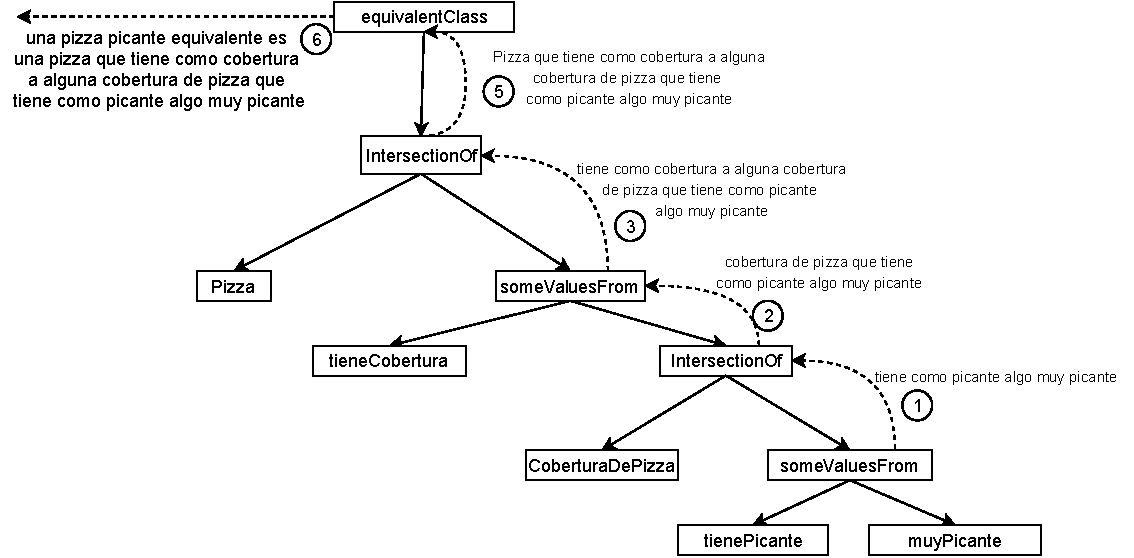
\includegraphics[width=\textwidth]{img/generacion_documento/verbalizacion_equivalentClass_spanish.pdf}
    \caption{Ejemplo gráfico de verbalización en lenguaje español.}
    \label{fig:ejemplo_verb_espaniol}
\end{figure}

\subsubsection{Axioma lenguaje inglés}
El ejemplo se tomó de la ontología Wine. El Axioma se corresponde al constructor \emph{owl:equivalentClass} sobre la clase \emph{CheninBlanc}. El contenido del axioma es el siguiente: 

\begin{verbatim}
EquivalentClasses(
    :CheninBlanc
    ObjectIntersectionOf(
        :Wine
        ObjectHasValue(
            :madeFromGrape
            :CheninBlancGrape)
        ObjectMaxCardinality(
        1
        :madeFromGrape)
    )
)
\end{verbatim}
La verbalización se muestra en la figura~\ref{fig:ejemplo_verb_ingles}.

Los pasos del proceso se encuentran enumerados desde el 1 al 4. Las gramáticas utilizadas son similares a las explicadas para lenguaje español, con la diferencia que los enlaces han sido traducidos a inglés.

Resulta conveniente explicar el paso Nº3 particularmente. El resultado de este paso es consecuencia de la intersección entre ``Wine'' y el resultado del paso 1 y 2. 
Como es una intersección de tres componentes, se procede a agrupar los componentes según su tipo, para luego unirlos a través de la conjunción ``y''. Dado que el operador \emph{hasValue} y \emph{minCardinality} retornan componentes de tipo SV, son agrupados juntos en una oración. Luego de agruparlos, se procede a realizar el proceso de agregación entre ambas, a través del cual se elimina el verbo ``made'' de la oración parcial construida en el paso 1. 

Por otro lado, la Clase Wine retorna un tipo T, por lo que queda aislado en una oración independiente. Estas agrupaciones resultan en el texto del paso Nº3.

La verbalización de este axioma da como resultado dos oraciones. Como ambas oraciones hacen referencia a la misma Clase, en el paso Nº4 ocurre un reemplazo del nombre de la Clase por una Expresión de Referencia. 

\begin{figure}
    \centering
    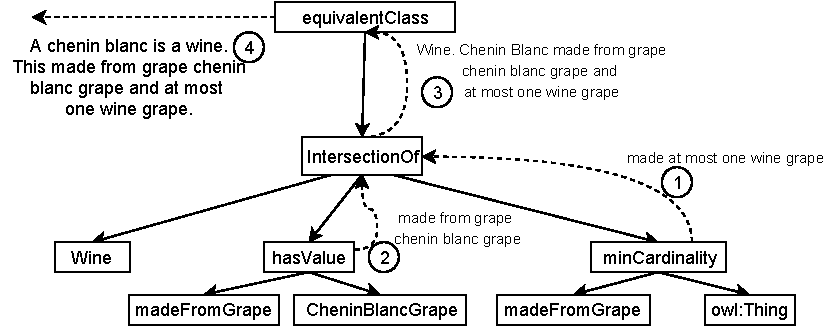
\includegraphics[width=\textwidth]{img/generacion_documento/verbalizacion_equivalentClass_english.pdf}
    \caption{Ejemplo gráfico de verbalización en lenguaje inglés.}
    \label{fig:ejemplo_verb_ingles}
\end{figure}

\subsection{Diagrama de clases}
En la figura \ref{fig:diagrama_clases_microplanificador} se puede ver el diagrama de clases asociado al módulo de micro planificación. Las subclases de \emph{OWLRestriction} tienen la capacidad de generar las oraciones parciales.

\begin{figure}[H]
    \centering
    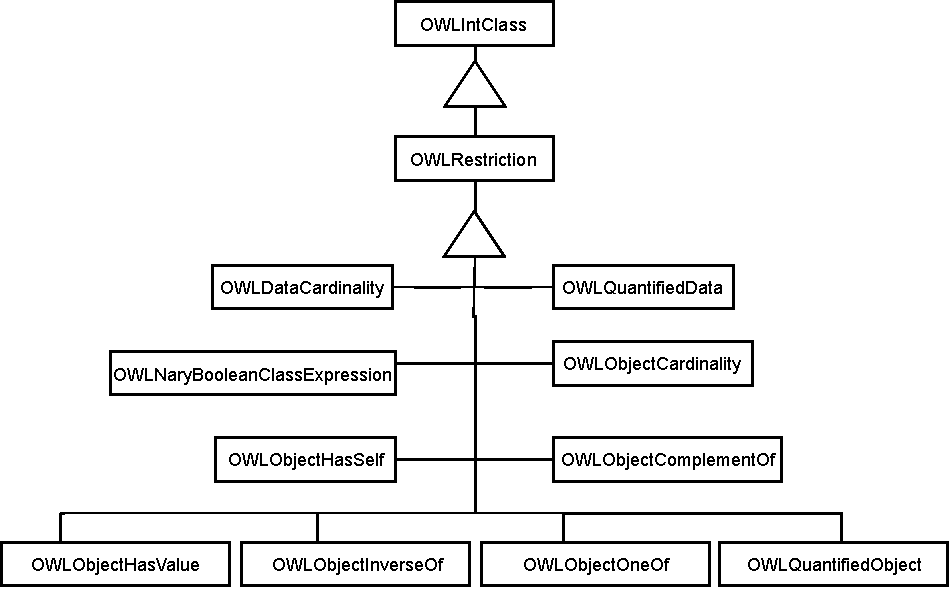
\includegraphics[width=10cm, height=7cm]{img/generacion_documento/diagrama_clases_microplanificador.pdf}
    \caption{Diagrama de clases del micro planificador.}
    \label{fig:diagrama_clases_microplanificador}
\end{figure}


\section{Implementación micro panning}

\subsection{Recursos usados}

\section{Diseño del realizador}
Este módulo se encarga de la tarea de diseñar la estructura final del documento, definiendo criterios para decidir si la información organizada se corresponde a secciones o párrafos.

Para simplificar el documento de salida, solo se consideraron dos niveles de información en el documento: el nivel más alto se corresponde a las secciones (o capítulos) y sub-secciones, y el nivel más bajo a los párrafos. 

Para llevar a cabo esta planificación, se buscó medir la información a verbalizar, por lo que se propuso como métrica principal a la cantidad de sentencias presentes en la descripción de un tópico. Este es el único parámetro para reconocer si a un tópico le corresponde una estructuración asociada a una sección o un párrafo. 

\subsection{Secciones y párrafos}
Una sección agrupa uno o más párrafos o sub-secciones, por lo que en una sección puede existir más de un tópico, con la condición de que esos tópicos tengan una relación, ya sea de hermanos o de hijos. Estas relaciones se obtienen de la estructura en árbol resultado de la macroplanificación. 

Para decidir si un tópico es planificado como una sección, se utiliza como medida la cantidad de sentencias que posee y si tiene algún tópico que a su vez deba ser planificado como una sub-sección.

El valor mínimo de sentencias usado para decidir si se planifica como una sección es de cinco sentencias. Para agregar flexibilidad, el algoritmo queda parametrizado con esta unidad de medida, por lo que puede personalizarse para variar la granularidad del texto de salida, forzando a crear secciones con diferentes cantidad de sentencias, lo que permite variar el diseño del documento de salida.

Otro criterio usado en complemento de la cantidad de sentencias, es si para un tópico existe algún sub-tópico que requiera planificarse como sección, permitiendo anidar secciones y sub-secciones. Este concepto de anidamiento de secciones se aplica recursivamente, por lo que la cantidad de niveles de secciones puede ser tan alto como la jerarquía de tópicos reconocidos en el árbol de tópicos. 

Cuando se reconoce a una sección, esta se incluye en el documento final como: \begin{itemize}
    \item una sección principal
    \item o como hija (sub-sección) de una sección existente.
\end{itemize}

Existe una relación directa entre las secciones y el árbol de tópicos. Todo tópico es una potencial sección, para ser planificado como tal, debe cumplir los criterios propuestos anteriormente. 

Si la cantidad de sentencias requeridas para ser considerado una sección, tiende a cero, la planificación del documento será fiel al árbol de tópicos; mientras que si la cantidad de sentencias tiende a infinito, la planificación perderá niveles de jerarquía, y únicamente contemplará como secciones a los tópicos del primer nivel del árbol.   

Si un tópico se planifica como párrafo, significa que ningún tópico que se encuentre en niveles inferiores de esa misma rama del árbol tiene aptitud para ser planificado como sección.

Si bien esto puede diseñar un documento con una gran cantidad de sub-secciones, siendo visualmente antinatural, ayuda a los humanos a reconocer y establecer relaciones entre los tópicos, siendo el objetivo principal no desaprovechar la semántica del dominio modelado, y teniendo como intención principal que el lector comprenda el dominio modelado en la ontología.

\section{Implementación del realizador}
El realizador está embebido dentro de la clase Section vista en la figura \ref{fig:diagrama_clases_macroplanificador}, en forma de funciones que implementan los criterios vistos para la definición del documento.


\section{Casos de estudio}

\subsection{Generación documento ontología Pizza}

\subsection{Generación documento ontología Wine}

\section{Conclusiones}

